% !TeX TXS-program:compile = txs:///lualatex

\documentclass[a4paper,11pt]{article}
\usepackage[revgoku]{cp-base}
\graphicspath{{./graphics/}}
%variables
\donnees[%
	classe=1\up{ère} 2M2,matiere={[SPÉ.MATHS]},typedoc=CHAP,numdoc=3,mois=Novembre,annee=2021
]

%formatage
\author{Pierquet}
\title{\nomfichier}
\hypersetup{pdfauthor={Pierquet},pdftitle={\nomfichier},allbordercolors=white,pdfborder=0 0 0,pdfstartview=FitH}
%fancy
\lhead{\entete{\matiere}}
\chead{\entete{\lycee}}
\rhead{\entete{\classe{} - \mois{} \annee}}
\lfoot{\pied{\matiere}}
\cfoot{\logolycee{}}
\rfoot{\pied{\numeropagetot}}

\begin{document}

\pagestyle{fancy}

\part{CH03 - Droites et fonctions affines - Exercices}

\smallskip

\exonum{0}

\medskip

Soit $(d)$ la droite d'équation $y=1,5x+5,5$.
%
\begin{enumerate}
	\item Déterminer le sens de variations de la droite $(d)$.
	\item Montrer que le point $A(1~;~7)$ appartient à $(d)$.
	\item Déterminer la valeur de $a$ pour que le point $B(a~;~8)$ appartienne à $(d)$.
	\item Le point $C(3,5~;~11,5)$ appartient-il à $(d)$ ? Justifier.
\end{enumerate}

\medskip

\exonum{1}

\medskip

Pour chacune des fonctions affines suivantes, déterminer son sens de variations, sa racine et son tableau de signes.
%
\begin{enumerate}
	\item $f_1(x)=4x-8$ ;
	\item $f_2(x)=-x+5$ ;
	\item $f_3(x)=3x+5$ ;
	\item $f_4(x)=-\dfrac23x+\dfrac14$.
\end{enumerate}

\medskip

\exonum{1}

\begin{enumerate}
	\item
	\begin{enumerate}
		\item Dans un repère orthogonal, placer les points $A(-1~;~-1)$, $B(1~;~3)$ et $C(2~;~2)$.
		\item Tracer les droites $(AB)$, $(AC)$ et $(BC)$ puis déterminer leur équation.
	\end{enumerate}
	\item Déterminer par lecture graphique une équation de chacune des droites tracées :
	\begin{center}
		\begin{tikzpicture}[x=0.8cm,y=0.8cm,xmin=-2,xmax=6,ymin=-3,ymax=4]
			\tgrillep[thin,lightgray]
			\axestikz* \axextikz*{-2,-1,...,5} \axeytikz*{-3,-2,...,3}
			\draw (0,0) node[below left=3pt,font=\sffamily] {0} (1,0) node[below=3pt,font=\sffamily] {1} (0,1) node[left=3pt,font=\sffamily] {1} ;
			%droites v1
			\clip (\xmin,\ymin) rectangle (\xmax,\ymax) ;
			\draw[ultra thick,red,samples=2,domain=\xmin:\xmax] plot (\x,{-\x+2}) ;
			\draw[ultra thick,blue,samples=2,domain=\xmin:\xmax] plot (\x,{3*\x-1}) ;
			\draw[ultra thick,ForestGreen,samples=2,domain=\xmin:\xmax] plot (\x,{2}) ;
			\draw[ultra thick,orange,samples=2,domain=\xmin:\xmax] plot (\x,{0.8*\x-2}) ;
			\draw[ultra thick,purple] (4,\ymin)--(4,\ymax) ;
			\draw[red] (2.5,-1.5) node[font=\large] {$(d_1)$} ;
			\draw[blue] (1.5,1.5) node[font=\large] {$(d_2)$} ;
			\draw[ForestGreen] (-1.5,1.5) node[font=\large] {$(d_3)$} ;
			\draw[orange] (-1.5,-2.5) node[font=\large] {$(d_4)$} ;
			\draw[purple] (4.5,0.5) node[font=\large] {$(d_5)$} ;
		\end{tikzpicture}
		\hspace{1cm}
		\begin{tikzpicture}[x=0.4cm,y=0.04cm,xmin=-4,xmax=14,ymin=-40,ymax=100,xgrille=2,ygrille=20]
			\tgrillep[thin,lightgray]
			\axestikz* \axextikz*{-4,-2,...,12} \axeytikz*{-40,-20,...,80}
			\draw (0,0) node[below left=3pt,font=\sffamily] {0} (2,0) node[below=3pt,font=\sffamily] {2} (0,20) node[left=3pt,font=\sffamily] {20} ;
			%droites v2
			\clip (\xmin,\ymin) rectangle (\xmax,\ymax) ;
			\draw[ultra thick,darkgray,samples=2,domain=\xmin:\xmax] plot (\x,{30*\x-20}) ;
			\draw[ultra thick,magenta,samples=2,domain=\xmin:\xmax] plot (\x,{-20/6*\x+80}) ;
			\draw[ultra thick,pink!50!black,samples=2,domain=\xmin:\xmax] plot (\x,{4*\x}) ;
			\draw[darkgray] (5,90) node[font=\large] {$(d_6)$} ;
			\draw[magenta] (13,30) node[font=\large] {$(d_7)$} ;
			\draw[pink!50!black] (5,30) node[font=\large] {$(d_8)$} ;
		\end{tikzpicture}
	\end{center}
\end{enumerate}

\medskip

\exonum{2}

\medskip

Dans un repère orthogonal, on considère les points $K(10\,;\,15,75)$ et $L(100,4\,;\,65,47)$.
%
\begin{enumerate}
	\item Déterminer, par \uline{calculs}, une équation de la droite $(KL)$.
	\item Le point de coordonnées $(50\,;\,37,85)$ appartient-il à la droite $(KL)$ ? Justifier.
\end{enumerate}

\newpage

\exonum{1}

\medskip

On considère les points $A(1~;~2)$, $B(2~;~8)$ et $C(5~;~26)$.
%
\begin{enumerate}
	\item
	\begin{enumerate}
		\item Montrer que le coefficient directeur de $(AB)$ vaut 6.
		\item Calculer le coefficient directeur de la droite $(AC)$.
		\item Déterminer une équation de la droite $(AB)$.
	\end{enumerate}
	\item Les points $A$, $B$ et $C$ sont-ils alignés ? Justifier.
\end{enumerate}

\medskip

\exonum{3}

\begin{enumerate}
	\item Donner le tableau de signes des expressions suivantes :
	\begin{enumerate}
		\item $(x-3)(2x-4)$ ;
		\item $-x(3x+4)$ ;
		\item $(x-2)(x+5)(7-7x)$ ;
		\item $\dfrac{2x+1}{(x-5)(x-1)}$ ;
		\item $\dfrac{-7(x+2)}{5-2x}$ ; \hfill{}{\footnotesize \textit{Ne pas oublier le $-7$ qui est  \og toujours négatif \fg}}
		\item $\dfrac{x^2+3}{(x-1)(x+4)}$.\hfill{}{\footnotesize \textit{On pourra utiliser le fait qu'un \og carré est toujours positif ! \fg}}
	\end{enumerate}
	\item Donner, après avoir \textit{transformé} si besoin, le tableau de signes des expressions suivantes :
	\begin{enumerate}
		\item $(x-3)(x-1) -2(x-3)(4x-7)$
		\item $3-\dfrac{5+x}{7x-13}$
		\item $x(x+2)(x-3)^2$
	\end{enumerate}
\end{enumerate}

\medskip

\exonum{3}

\begin{enumerate}
	\item Résoudre (directement avec un tds), les inéquations suivantes :
	\begin{enumerate}
		\item $(x-3)(2x+4) \pg 0$ ;
		\item $3x(x+1)(7+x) < 0$ ;
		\item $\dfrac{x+3}{2x+8} \pp 0$ ;
		\item $\dfrac{x(x+2)}{x+1} > 0$.
	\end{enumerate}
	\item Résoudre, en transformant si besoin, les inéquations suivantes :
	\begin{enumerate}
		\item $7x+3 \pp 2$ ;
		\item $(x+1)(x-2) < (x+1)(4x+5)$ ;
		\item $\dfrac{x+1}{x+2} < 2$.
	\end{enumerate}
\end{enumerate}

\medskip

\exonum{3}

\medskip

Retrouver, par \og calculs \fg{} le résultat donné par \cxcas{Xcas}, logiciel de calcul formel :
%
\begin{center}
	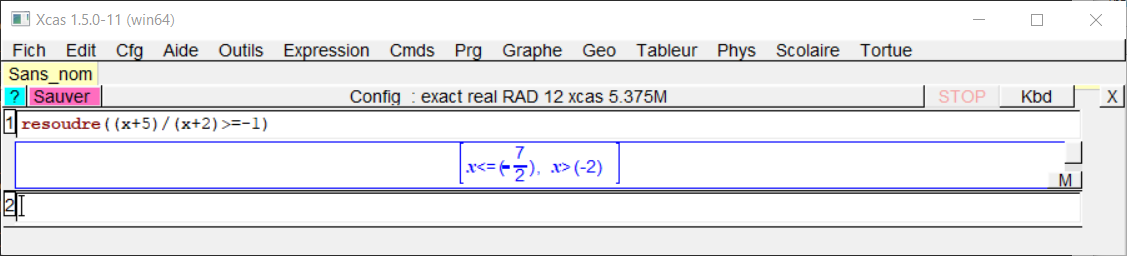
\includegraphics[scale=0.7]{chap03_td_xcas}
\end{center}

\end{document}